%\dropchapter{0.4in}
\chapter{The CMS experiment at CERN's accelerator complex} \label{chp:CERN}
%\epigraphhead[70]{\epigraph{\textit{If I could remember the names of all these particles, I'd be a botanist.}}{Enrico Fermi}}
%\undodrop

The Standard Model of elementary particle physics, for which the main successes and shortcomings have been discussed extensively in Chapter~\ref{chp::SM}, results in very precise predictions. However it is only acknowledged as an effective theory up to an energy scale of about $1 \TeV$. Physics beyond this energy is studied with specific high-energetic particle colliders such as the Large Hadron Collider (LHC) located at CERN (European Council for Nuclear Research) near Geneva. The LHC provides proton-proton collisions at a record-breaking energy and is currently the world's most energetic particle collider.\\
Several different experiments surround the LHC, each with a specific physics goal ranging from general high-luminosity physics to dedicated plasma-studies and even long-lifetime neutrino interactions.
In this chapter attention will mainly be devoted to the Compact Muon Solenoid (CMS) experiment, which is the LHC general-purpose experiment used for recording the data processed within this thesis.

\section{The Large Hadron Collider}
The need for a particle collider with the dimensions of the LHC was driven by a quest to understand the nature of the electroweak symmetry breaking, for which the Brout-Englert-Higgs mechanism is presumed to be responsible, and to investigate physics at the $\TeV$ scale.
Such high energies can only be achieved when state-of-the-art technology is used for both accelerating and colliding the particles, and for recording the provided interactions.
\\

When the design of the LHC machine was approved in 1994 it was decided to reuse the existing $26.7 \km$ Large Electron Positron (LEP) tunnel, previously excavated in the 1980's and positioned between 45m and 150m below the Earth's surface.
Avoiding the construction of a new tunnel was a huge cost-saver but presented some stringent limitations on the machine's design. For example the space limitation in the tunnel compelled the use of so-called twin-bore magnets where both proton rings are contained within a single magnet structure.
\\
The LHC is designed to provide proton-proton collisions with a beam energy of $7 \TeV$ each, resulting in a centre-of-mass energy $\sqrt{s}$ of $14 \TeV$. This is a seven-fold energy increase compared to the previous most energetic particle collider: the Tevatron which yielded proton-antiproton collisions between 1983 and 2011. In order to reach these extreme energy conditions the LHC exploits the presence of the extensive accelerator complex at CERN to gradually increase the beam energy. 
\\
When the proton beams are circulating within the LHC at the desired beam energy they can be steered in order to collide head-on in the dedicated interaction regions. Of the eight interaction regions existing in the LEP tunnel only four have actually been equipped with particle detectors for the LHC data-taking. The ATLAS~\cite{AtlasDetectorPaper} and CMS~\cite{CMSDetectorPaper} experiments are the two largest ones and are intended as general-purpose detectors studying a broad range of physics processes while the ALICE~\cite{AliceDetectorPaper} and LHCb~\cite{LHCbDetectorPaper} experiments search for a specific type of physics interactions. The ALICE experiment serves mainly for heavy-ion physics while LHCb is dedicated to heavy-flavour physics.
\\
Within this thesis data collected at the CMS detector during the first era of data-taking has been analysed, which started in March 2010 and continued until December 2012. These collisions did not take place at the design beam energy of $7 \TeV$ but at a reduced energy of $3.5 \TeV$ and $4 \TeV$ for the 2010-2011 and 2012 data-taking, respectively.

\subsubsection{The LHC's design, driven by the LEP legacy}
The design of the LHC project, approved in 1994 by the CERN council, is characterised by both the predefined physics reach and the available infrastructure at the CERN accelerator complex.
The obligation to reuse the existing LEP tunnel introduced some additional challenges on top of the ones following from the extremely high energy regime. 
\\

The decision to accelerate protons instead of electrons, as was the case for LEP, was lead by the extremely high beam energy desired for the parton interactions. Less massive particles loose a significant amount of their energy due to synchrotron radiation when travelling at high speed in a circular orbit. With velocities close to the speed of light, as foreseen at the LHC, this energy loss would represent a limiting factor for the final energy reachable when accelerating electrons. This effect is almost negligible for protons.
\\
The physics goals set by the LHC also compelled to step away from the approach adopted at the Tevatron: providing collisions between protons and anti-protons. This because the desired number of collisions, represented by the luminosity $\mathcal{L}$, would not be attained when using anti-protons. The design luminosity was fixed to reach a record-breaking value of $10^{34} \cm^{-2} \s^{-1}$, corresponding to around 1 billion interactions per second. Such a high rate of collisions is only feasible when the partons are confined into dense bunches of about $10^{11}$ particles.
In order to fulfil these challenging conditions the interacting partons need to be produced in adequate amounts, which is not realisable for anti-protons.
As a result is was decided to provide proton-proton interactions at the LHC.
%Hence the decision to provide/yield proton-proton interactions at the LHC.
\\
The relatively small circumference of the LHC tunnel combined with the extremely high velocity of the circulating protons compels the use of superconducting magnets. Although superconductivity was already used extensively in previous accelerators, the LHC pushed the existing technology to a new level by operating at a record-breaking temperature of $1.9 \K$ resulting in the production of a $8.33 \Tesla$ strong magnetic field. 
These superconducting dipole magnets, of which 1232 exist in the LHC, are responsible for bending the proton trajectory.
\\
However the use of particles with the same electric charge introduces an additional challenge since two separate magnetic fields are required to bend the protons in opposite directions. For the LHC this lead to the development of twin-bore magnets consisting of two separate beam pipes each surrounded with individual superconducting coils within the same mechanical structure.
A schematic cross-section of such an LHC dipole magnet is given in Figure~\ref{fig::LHCDipole}.
\begin{figure}[h!t]
 \centering
 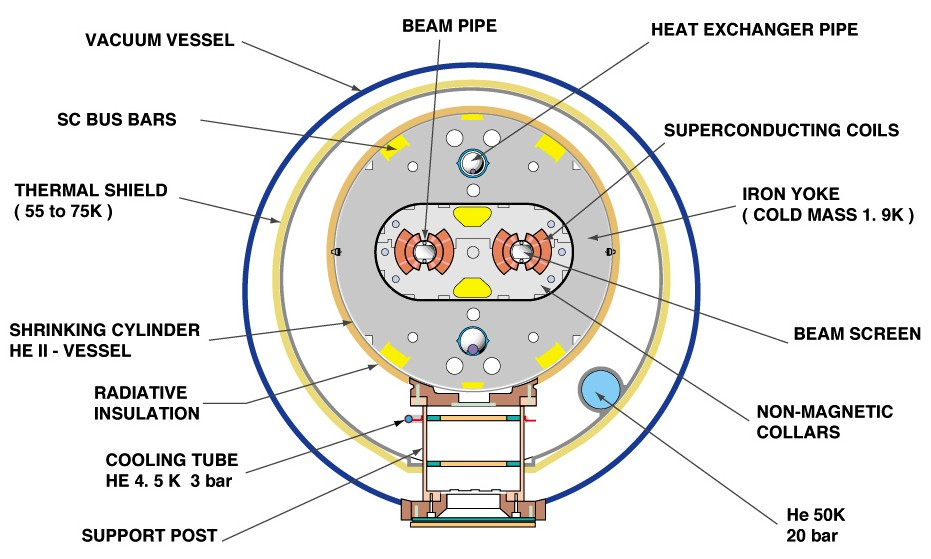
\includegraphics[width = 0.6 \textwidth]{Chapters/Chapter2_CERN/Figures/lhc-pho-1998-341.jpg}
 \caption{Cross-section of an LHC dipole magnet with the twin-bore design.}%Taken from http://cds.cern.ch/record/841539/
 \label{fig::LHCDipole}
\end{figure}

The tunnel of the Large Hadron Collider is not a perfect circle but consists of eight arcs and eight straight sections.
The 15$\m$ long dipole magnets are located in the arcs and are responsible for preserving the circular orbit of the protons.
The actual accelerator of the protons is provided by the dedicated radio-frequency (RF) cavities, which are positioned in one of these straight sections.
A second type of magnets, so-called quadrupole magnets, are located throughout the entire tunnel and ensure that the beams remain aligned and do not drift apart. These quadrupole magnets are able to squeeze the beam either vertically or horizontally and are also installed just before the different detectors where they provide an additional squeezing to increase the chances on a collision.

\subsubsection{The LHC injection chain}
The LHC does not only reuse the existing LEP tunnel it also benefits strongly from the complete accelerator complex present at CERN in order to reach the record energy of $7 \TeV$. 
The protons run through a series of interconnected linear and circular accelerators and are only passed on to the next in line once they attain the maximum speed possible for that specific accelerator. A schematic overview of the sequence used for the proton acceleration at the LHC is given in Figure~\ref{fig::LHCChain}.\\
The entire LHC injection chain starts with a box of hydrogen atoms from which protons are electrically stripped and accelerated to an energy of about 50 $\MeV$ when passing through the Linac2.
Following to this linear acceleration, the protons are injected into the first circular accelerator, the Proton Synchrotron Booster (PSB), where they remain until reaching an energy of $1.4 \GeV$.
Once the protons are energetic enough they will be shot into the Proton Synchrotron (PS) and become accelerated to $25 \GeV$, the maximum speed reachable by the PS.
Afterwards they are finally inserted in the last accelerator of the injection chain, which is the Super Proton Synchtrotron (SPS).
The SPS is responsible for accelerating the protons up to $450 \GeV$ after which the LHC is capable of accelerating them further until the nominal energy of $7 \TeV$.
\begin{figure}[h!t]
 \centering
 \includegraphics[width = 0.99 \textwidth]{Chapters/Chapter2_CERN/Figures/CERN_Chain.pdf}
% 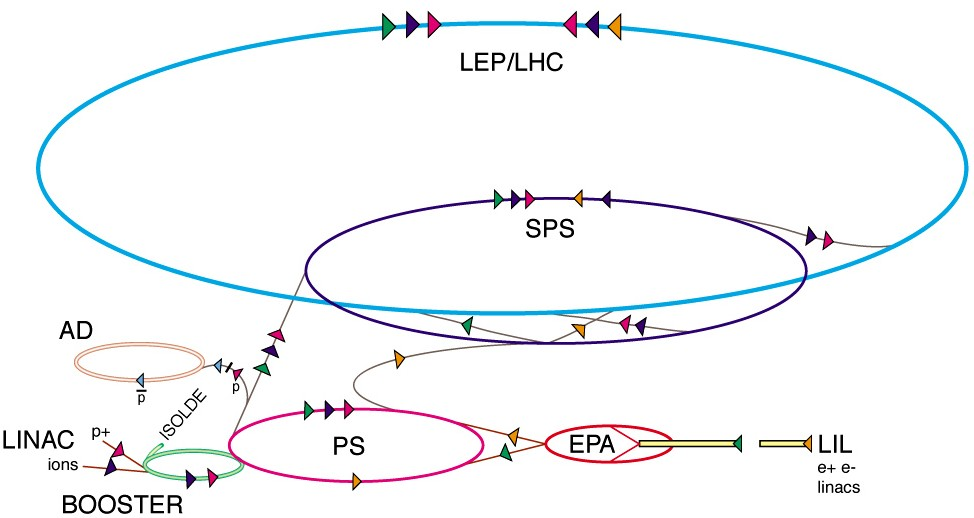
\includegraphics[width = 0.8 \textwidth]{Chapters/Chapter2_CERN/Figures/CERNAcceleratorComplex_Few.jpg}
 \caption{Detailed overview of the LHC injection chain.} \label{fig::LHCChain}
\end{figure}

The protons accelerated at the LHC are confined in large proton bunches since this significantly increases the possibility of observing at least one proton-proton interaction during a single bunch crossing. 
The design of the LHC is optimised for providing $pp$ collision with not only a record-breaking beam energy, but also with the highest luminosity ever recorded. In order to reach the design luminosity the LHC should store multiple proton bunches in a so-called bunch train with the smallest separation possible. 
This is a common technique adopted in most accelerators with the important difference that the LHC can reach much smaller bunch separations than ever before, up to $25 \ns$.
\\
The proton bunches are created by the RF cavities responsible for accelerating the protons, a process which starts already during the first stages of the LHC injection chain.
These type of cavities produce a resonant electromagnetic wave that oscillates at a given frequency and accelerates the protons up to an ideal energy.
Hence inverting the electromagnetic field ensures that the protons become organised into discrete packets since protons travelling too fast will undergo a deceleration while those arriving late will feel an additional push.
The adopted accelerator sequence is constructed such that each successive accelerator is capable of containing more bunches allowing a gradual filling of the bunch train.

\subsubsection{Particle detectors}
The Large Hadron Collider has dedicated areas in the tunnel where beam crossings are provided and particle detectors are placed in order to measure the particle activity present during proton-proton collisions. The four interaction regions utilised by the main LHC experiments CMS, LHCb, ATLAS and ALICE are represented as yellow blobs in Figure~\ref{fig::LHCChain}. 
\\
As shortly mentioned before the two largest experiments are the two general-purpose experiments CMS and ATLAS. They are both designed to cover a wide range of physics processes and are constructed following an onion-layered structure around the interaction point to avoid particles escaping detection. The main difference between the two experiments is the shape of the magnet: ATLAS uses a toroidal magnet while CMS adopted a solenoid configuration. 
%The magnet is one of the crucial parts of any particle detector since it allows to extract useful information from a particle's track. 
More detail about the CMS detector and the different layers it contains will be discussed in Section~\ref{sec::CMS}.
\\
The two smaller experiments, ALICE and LHCb, tend to focus on a dedicated type of physics processes and are optimised as such. The ALICE experiment is a heavy-ion detector which is interested in the Pb-Pb collisions also provided by the LHC machine. It aims to gather information about the quark-gluon plasma, a phase of matter where the quarks and gluons are no longer confined in hadrons. The LHCb experiment focuses on heavy flavour physics and will try to explain why the universe seems to constitute almost entirely of matter and not of anti-matter. The design of this detector is rather distinctive since it does not follow the standard shape of an enclosed detector positioned symmetrically around the interaction region, but instead consists of a half-open structure designed to accurately measure forward particles.
\\
The CERN site contains many other smaller experiments which try to grasp the physics behind some of the remaining unsolved mysteries and hope to result in useful future applications. 
Specific for the LHC tunnel are the three experiments which are located in the vicinity of one of the main particle detectors sharing the same experimental cavern.
The first one is the TOTEM~\cite{TotemDetectorPaper} experiment, which is placed close to the CMS detector along the beampipe and is designed to investigate the proton structure %\footnote{Definitely certain that 'structure' is good to be used??} 
in the very forward region. The LHCf~\cite{LHCfDetectorPaper}, installed near ATLAS, will also focus on physics in the very forward region, but aims to better understand hadron interaction models used in the simulation of high-energy cosmic rays.
The last experiment, MOEDAL~\cite{MoedalDetectorPaper} is deployed around the LHCb interaction region and will try to detect the magnetic monopole, a hypothetical particle with magnetic charge.

\subsubsection{Run-I (2010-2012) data taking}

The LHC is  designed to provide proton-proton collisions with a centre-of-mass energy $\sqrt{s}$ = 14 $\TeV$ and the first proton beams made circulating in September 2008 were indeed configured for these conditions. However a mechanical incident on 19 September 2008 delayed the observation of the first LHC collisions to March 2010 and forced the LHC to run at a reduced energy of $3.5 \TeV$ per beam. The same beam energy was kept during the 2011 run and was only slightly increased during the final year of the Run-I data taking period in order to provide collisions at $\sqrt{s}$ = $8 \TeV$. In between the proton-proton runs dedicated ion-ion or proton-ion collisions were scheduled for the specific heavy-ion studies performed at the different experiments.
\\
The number of collisions produced during the proton-proton collisions can be represented by the integrated or instantaneous luminosity, expressed in terms of $\pbI$. The difference between the integrated and instantaneous luminosity lies in the considered time span. The instantaneous luminosity is the number of collisions provided by the LHC each second, while the integrated luminosity is the accumulated number of interactions during a longer period of time. Figure~\ref{fig::InstLumi} contains the maximum instantaneous luminosity delivered to the CMS experiment for $pp$ collisions for each day of the three years long Run-I data-taking period.
Summing the daily contributions results in a total value for the integrated luminosity during the three years of Run-I of respectively, $44.2 \pbI$, $6.1 \fbI$ and finally $23.3 \fbI$.
\begin{figure}[h!t]
 \centering
 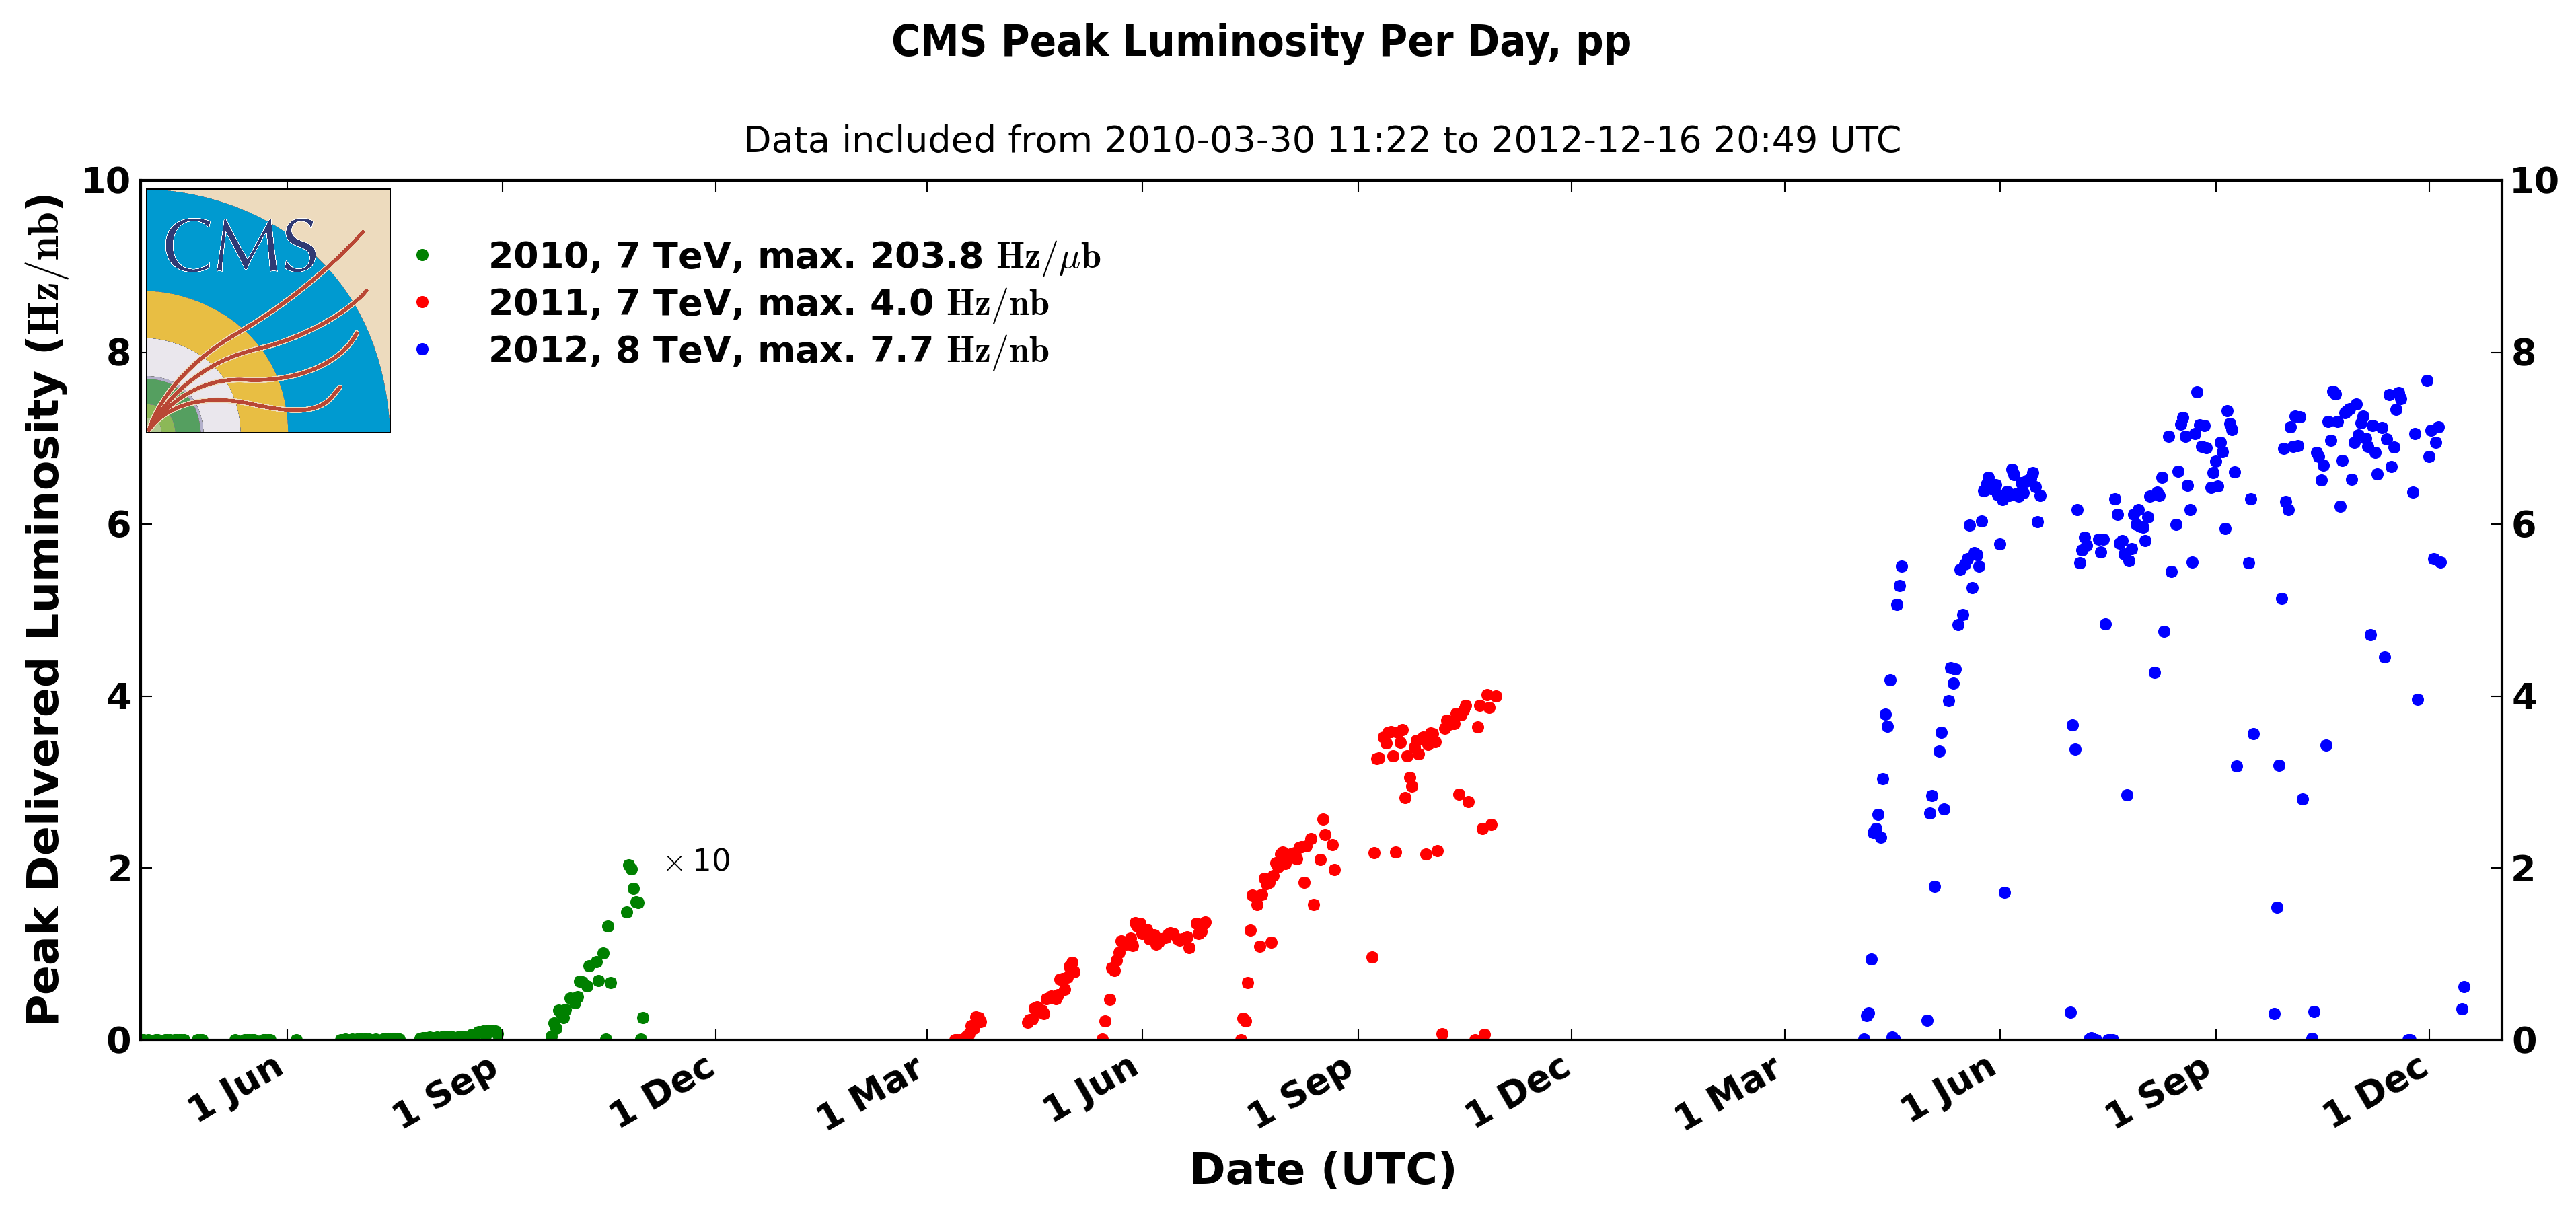
\includegraphics[width = 0.95 \textwidth]{Chapters/Chapter2_CERN/Figures/InstanteneousLumi_FullRunI.png}
 \caption{Overview of the daily peak luminosity delivered to the CMS detector during the 2010-2012 data-taking period.} 
 \label{fig::InstLumi}
\end{figure}

\section{The Compact Muon Solenoid detector}\label{sec::CMS}

One of the two main-purpose particle detectors of the Large Hadron Collider is the Compact Muon Solenoid (CMS) experiment designed to perform a wide variety of physics measurements. Therefore the specifications of the CMS experiment follow from the LHC physics program goals requiring good identification and momentum resolution throughout the entire detector.
In order to efficiently measure all the different particles emerging from the interaction point, the CMS apparatus~\cite{CMSTDR} consists of four separate subdetectors which are all optimised to identify specific types of particles: a tracking detector, an electromagnetic and hadronic calorimeter, and a muon system. 
The first three layers of the CMS detector are confined within the high-field superconducting solenoid magnet of $3.8 \Tesla$, as depicted in Figure \ref{fig::CMSFig}. 
From a geometric perspective each of the subdetectors consists of a cylindrical barrel part centred around the interaction point for which both ends are closed hermetically by an endcap structure.
\begin{figure}[h!t]
 \centering
 \includegraphics[width = 0.95 \textwidth]{Chapters/Chapter2_CERN/Figures/cms_OverviewCropped.pdf}%Taken from https://cms-docdb.cern.ch/cgi-bin/PublicDocDB/RetrieveFile?docid=11514&version=1&filename=cms_120918_03.png
 \caption{CMS layout with all subdetectors clearly visible.} \label{fig::CMSFig}
\end{figure}

The layout of the CMS detector is mainly driven by the superconducting solenoid since the subdetectors positioned inside the magnet bore need to be as compact as possible without any loss of granularity. In addition the size of the muon system is restricted to four stations because of the magnet's return field.
\\
The tracking detector is placed closely around the beam pipe and consists of a separate silicon-based pixel part and a strip detector as will be explained in Section~\ref{sec::Tracker}, in order to guarantee track reconstruction in the high density environment close to the interaction point.
Around the tracking detector the electromagnetic calorimeter (ECAL) and hadronic calorimeter (HCAL) are positioned, which are responsible for accurately measuring the energy of the particles emerging from the interaction region. More detail about the characteristics of the calorimeter systems will be given in Section~\ref{sec::CAL}. Finally, surrounding the magnet coil, the muon chambers interleaved with the steel return yokes can be found. This part of the CMS detector, discussed in detail in Section~\ref{sec::MuonChamber}, provides an accurate muon identification, crucial for distinguishing promising muon final state signatures from the extensive background. 
The overall dimensions of the full CMS detector are a total length of $21.6$ m and a diameter of $14.6$ m resulting in a total weight of 12 500 tons.
\\
\\
%The design of the CMS experiment is \textbf{also} optimized for the reconstruction of neutrino's, which cannot be measured directly and hence only appear in the form of missing energy, by ensuring a hermetically closed detector. This resulted\footnote{Is this really the motivation why a barrel and endcap design has been adopted??} in the construction of a cylindrical barrel part located centrally with respect to the interaction point and an endcap part represented by a sort of disklike closure componenents for each of the different subdetectors.
The CMS experiment has adopted a proper coordinate system for which the origin is centred at the nominal collision point within the detector. The $y$-axis is pointing upwards and the $x$-axis radially inwards toward the centre of the LHC. Hence, according to the right-hand rule, the $z$-axis follows along the anticlockwise-beam direction. This coordinate system can easily be converted into a spherical coordinate system where the azimuth angle $\phi$ is measured in the $x$-$y$ plane and the polar angle $\theta$ from the $z$-axis. 
From this coordinate system the pseudo-rapidity $\eta$ can be derived, a variable used extensively in accelerator physics since it has the advantage to be invariant with respect to Lorentz boosts along the beam axis. Therefore this variable, defined as,
\begin{equation} \label{eq::PseudoRapidity}
 \eta = - \ln \tan \frac{\theta}{2}
\end{equation}
is used to describe the angle of a particle with respect to the $z$-axis. The pseudo-rapidity is closely related to the rapidity, denoted with the symbol $y$ and defined in Equation (\ref{eq::rapidity}). Since this variable requires both the energy and the total momentum of a particle to be known, the rapidity is more challenging to determine. However in the case of high-energy collisions, both quantities are almost identical.
\begin{equation}\label{eq::rapidity}
 y = \frac{1}{2} \ln \left( \frac{E+p_{z}}{E - p_{z}} \right)
\end{equation}

The Large Hadron Collider is able to provide a bunch-crossing rate of about 40$\unit{MHz}$, however, the current state-of-the-art computer systems are not capable of handling such a large amount of data.
Hence the CMS experiment has been equipped with a dedicated multi-layered online event-selection system and uses a specialised computing system to store, transfer and manipulate the recorded data as will be explained in Section~\ref{subsec::L1HLT}.
The capability of the CMS detector to efficiently perform this complex data handling is discussed in Section~\ref{subsec::CMSPerf}.

\subsection{The silicon tracking apparatus}\label{sec::Tracker}
The CMS tracking detector is located at the most inner point of the magnet bore close to the interaction point and is hence exposed to the harsh radiation environment produced by the proton-proton collisions. In order to survive these challenging conditions and still be capable of providing fast and accurate read-out of the particle's hits, it was decided to fully equip this tracking detector with active silicon, making it the largest silicon tracker ever constructed.
\\
For the CMS tracking apparatus two different detection techniques have been adopted.
The most inner part of the detector consists of pixel cells of size 100 $\times$ 150$ \unit{\mu m}^{2}$, capable of achieving similar track resolution in both $r-\phi$ and $z$ direction, while the outer part contains silicon micro-strip sensors with diverse track resolution. 
This choice is motivated by the varying particle flux conditions throughout the tracking detector, which start out rather extreme at low radii but become more sensible when moving further away from the interaction region. 
Therefore the technology used in the first layers of the CMS tracker should be able to identify individual particle hits in a very dense track regime, which is feasible for silicon micro-strips. However the use of silicon strips is sufficient in the outer regions of the tracking detector where the track rate is significantly lower.
From Figure~\ref{fig::CMSTracker}, which shows the geometry of the CMS tracker, the two structures are clearly visible together with the general subdetector layout containing central barrel layers closed with endcap disks allowing a larger $\eta$-coverage.
\begin{figure}[h!t]
 \centering
 \includegraphics[width = 0.99 \textwidth]{Chapters/Chapter2_CERN/Figures/CMS_TrackerLayout_Overview-eps-converted-to.pdf}
 %\includegraphics[width = 0.99 \textwidth]{Chapters/Chapter2_CERN/Figures/TrackerLayout_Color.pdf}(If color one is used, the difference between blue (=3-D hit positions) and black (=2-D hit positions) need to be understood and explained!!!)
 \caption{Schematic cross-section of the CMS tracking detector.} \label{fig::CMSTracker}
\end{figure}

The pixel part of the tracker subdetector consists of three cylindrical barrel layers (BPix) placed at radii 44, 73 and 102$\mm$ and two endcap disks (FPix) positioned at z = $\pm$ 345 and $\pm$ 465$\cm$ on each side. The barrel layers itself are 570$\mm$ long and thus extend up to $z$ = $\pm$ 285$\cm$ resulting in, combined with the chosen positioning of the two endcap disks, at least three tracking points for almost the full pseudo-rapidity range. The silicon strip subdetector is further divided into an inner and outer part, both of which follow the barrel-endcap structure. The Tracker Inner Barrel (TIB) contains 4 concentric barrel layers located at radii 255.0, 339.0, 418.5 and 498.0$\mm$ which extend from -700$\mm$ to +700$\mm$ along the beampipe. The Tracker Inner Disks (TID) are the endcap configuration for the inner strip detector and are each made up of 3 disks placed between $\pm$ 800 and $\pm$ 900$\mm$ in z. Finally the Tracker Outer Barrel (TOB) and Tracker End Cap (TEC) further extend the overall dimensions of the CMS tracker detector to a diameter of 2.4$\m$ and a length of 5.4$\m$ by adding 6 detection layers and 9 disks.

\subsubsection*{Hit and track reconstruction in the pixel and strip tracker}

This track reconstruction algorithm is a computational complex and iterative process. It is designed to start from the innermost hit of the pixel detector and proceed outwards layer by layer. Hence this algorithm is active in the most dense environment of the tracker and therefore requires an efficient search for hits and a fast trajectory propagation. The track reconstruction within CMS is defined as the Combinatiorial Track Finder~\cite{TrackAndPVReco} (CTF) and can be decomposed into four different steps: seed generation, pattern recognition, ambiguity resolution and track fitting.
%The local reconstruction is performed prior to the iterative tracking and clusters energy deposits by combining neighbouring pixels or strips which fulfill specific signal over noise (S/N) requirements. The cluster position is determined from the charge-weighted average or from the cluster edges in the case of the strip or pixel detector, respectively.
\begin{myindentpar}
  \begin{description}
    \item[Seed generation] \hfill \\
    This step of the track reconstruction provides initial trajectory candidates from pairs of pixel hits. 
    The starting trajectory parameters and associated uncertainty can be determined from only five parameters since the magnetic field remains quasi-uniform in a large part of the tracker volume. Hence either three hits or two hits combined with a beam spot constraint are sufficient to determine the seed trajectory of potential tracks.
    \item[Pattern recognition or track finding] \hfill \\
    This part of the CTF algorithm determines which hits are compatible with the seed trajectory using a combinatiorial Kalman Filter~\cite{KalmanFilter} method.
    It starts by scanning for layers likely to be intersected by the track candidate. Then the trajectory parameters are extrapolated to this layer and the compatible hits are identified. Finally the track parameters are updated by adding one of the compatible hits and the procedure is repeated until the outermost layer is reached.
    \item[Ambiguity resolution] \hfill \\
    Since for each of the compatible hits the trajectory candidates are grown in parallel, a single seed can result in multiple tracks or two identical tracks can originate from a different seed. This possible double-counting can be avoided by excluding specific tracks based on the number of hits shared among them. 
    \item[Track fitting] \hfill \\
    The remaining mutually exclusive trajectory candidates are recalculated during the last step of the iterative tracking algorithm. It uses a Kalman Filter method on the full list of hits starting from the innermost one. Afterwards a smoothing stage is applied in the form of an outside-in Kalman Filter based on the result of the first one. This approach yields optimal estimates of the parameters.
  \end{description}
\end{myindentpar}
Executing this CTF sequence multiple times and removing the hits associated with reconstructed tracks after each iteration significantly decreases the combinatorics. % combinatiorial complexity. 
By first identifying the more straightforward track candidates the streamlined collection of unmatched hits allows the recovery of tracks that slightly deviate from the simplified pattern. 
Therefore the track reconstruction algorithm is implemented such that first the prompt tracks are identified and only afterwards the ones originating from outside the luminous region of the proton-proton collisions.
%The algorithm is defined in a flexible way permitting it to be adapted to possible changing data-taking conditions.

The performance of the track reconstruction is outstanding, and muons are reconstructed better than any other charged particle~\cite{TrackAndPVReco}. For isolated muons with 1 $<$ $\pT$ $<$ 100$\GeV$ the tracking efficiency is higher than 99$\%$ for the entire $\eta$-range of the tracker and does not depend on $\pT$. The transverse momentum resolution for a muon with $\pT$ = 100$\GeV$ and $\vert \eta \vert$ $<$ 1.6 is of the order of 2-3$\%$ but quickly deteriorates for higher pseudo-rapidity values.
The efficiency for charged hadrons in $t\bar{t}$ events varies between 85 and 95$\%$ depending on the $\pT$ and $\eta$ value. %, and the \textit{What is it for this??? Only given separately for barrel/endcap/transition region ...}

\subsubsection*{Primary vertex reconstruction}
Once the full collection of reconstructed tracks is recovered the location and corresponding uncertainty of the associated proton-proton interaction vertices should be determined. Since only prompt tracks originating from near the interaction region are relevant for the primary vertex, these type of tracks need to be selected first. Afterwards the tracks that appear to originate from the same interaction vertex are clustered based on their $z$-coordinates. Finally the actual vertex fitting can be applied on the candidates which contain at least two tracks using an adaptive vertex filter~\cite{AdaptiveVertexFitting}. This fitting procedure computes the vertex parameters and assigns a weight to each track in the vertex, reflecting the probability that it actually belongs to the considered vertex.
\\

The complete primary vertex reconstruction results in an accurate measurement of the position of the primary vertices. For events with a reconstructed jet with transverse energy $\ET$ $>$ 20$\GeV$ the obtained resolutions are about 10$\unit{\mu m}$ in $x$ and $y$, and 12$\unit{\mu m}$ in $z$~\cite{TrackAndPVReco}. 

\subsection{The calorimetry subdetectors}\label{sec::CAL}
Any charged particle emerging from the interaction point will be detected by the tracker detector and its trajectory will be reconstructed. However in order to fully identify the observed particle this information should be combined with the measured energy deposits, a task performed by the electromagnetic and hadronic calorimeters. The ECAL is designed to measure the parton showers produced by electrons and photons while the HCAL will absorb the hadron and neutron showers.

\subsubsection{The electromagnetic calorimeter}
The ECAL is a hermetic homogeneous detector made of lead tungstate (PbWO$_{4}$) crystals, which ensures the detector to be fast, fine in granularity and radiation resistant. 
%As a downside, the yield of these type of cristals is rather low such that photodetectors are needed to detect the scintillator light produced when particles traverse the calorimeter cells. 
The ECAL subdetector contains in total 75 848 of lead tungstate scintillating crystals, of which 
61 200 are placed in the barrel part (EB) while the remaining are equally distributed among the two endcap structures (EC). % holds 7 324 of these crystals.
The pseudo-rapidity coverage of the EB is $\vert \eta \vert$ $<$ 1.479, which is further extended by the two endcaps to $\vert \eta \vert$ $<$ 3.0, as can be seen in Figure~\ref{fig::ECAL}. The crystals used in the two subdetector parts vary slightly, for the barrel crystals with a front-face cross section of 2.2 $\times$ 2.2$\cm^{2}$ with a total length of 23$\cm$ were constructed while for the endcap these values take 2.86 $\times$ 2.86$\cm^{2}$ and 22$\cm$, respectively.
\begin{figure}[h!t]
 \centering
 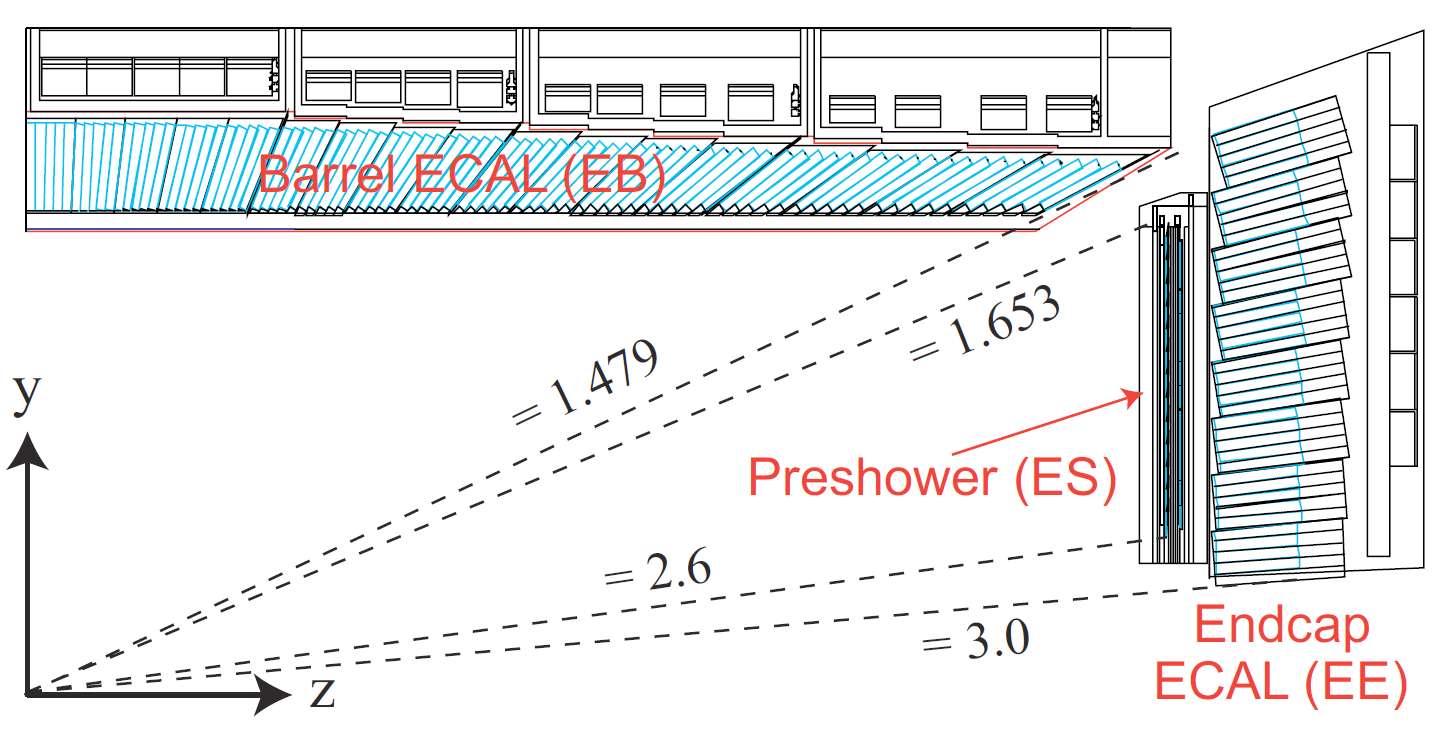
\includegraphics[width = 0.99 \textwidth]{Chapters/Chapter2_CERN/Figures/Experimental_Apparatus_ECAL.pdf}
 \caption{Overview of one quarter of the electromagnetic calorimeter with the different substructures and their respective pseudo-rapidity coverage.} \label{fig::ECAL}
\end{figure}

The ECAL contains besides the barrel and endcap an additional third substructure: the Preshower (ES). This is a sampling calorimeter consisting of lead radiators combined with silicon strip sensors specifically designed to identify and reject signals originating from neutral pions and minimum ionising particles. % (\textit{Is this last part also correct??}) 
The ES is only 20$\cm$ thick and is restricted to the $\vert \eta \vert$ coverage between 1.653 and 2.6. 
%Originally it was foreseen to also position a preshower calorimeter in front of the barrel detector but this appeared unrealistic due to the limited space available inside the magnet bore.

The energy for photons and electrons can be measured very precise with the electromagnetic calorimeter.
Their energy resolution has been measurered with electrons originating from Z-boson decays, for which resolutions of 2$\%$ are obtained in the central region and 2-5$\%$ elsewhere~\cite{ECALResolution}.

\subsubsection{The hadronic calorimeter}
The HCAL subdetector surrounds the electromagnetic one and is the last part of the CMS experiment confined within the solenoid.
It is a brass/scintillator calorimeter, motivated by the fact that brass is an efficient hadron absorber on a short scale and that the use of scintillating tiles is interesting when only limited space remains for the active medium. The geometrical design of the hadronic calorimeter is depicted in Figure~\ref{fig::HCAL} and also consists of a barrel and endcap part.
\begin{figure}[h!t]
 \centering
 \includegraphics[width = 0.95 \textwidth]{Chapters/Chapter2_CERN/Figures/cms_HCALLayout_Cropped.pdf}
 \caption{Layout of the hadronic calorimeter. (crop figure)} \label{fig::HCAL}
\end{figure}

The barrel (HB) consists of 17 scintillator plates, each 3.7$\mm$ thick, interleaved with brass plates of 5$\cm$. The only exception is found for the first scintillating plate, which has a thickness of 9$\mm$ and is designed to actively sample the particles showering due to the interaction with the support material placed between the ECAL and HCAL. The individual scintillator tiles have a size of $\Delta \eta$ $\times$ $\Delta \phi$ = 0.087 $\times$ 0.087, cover an overall pseudo-rapidity range of $\vert \eta \vert$ $<$ 1.4 and are contained within radii 1777$\mm$ and 2876.5$\mm$. The endcaps (HE) are made up of 19 scintillator plates with the same thickness and brass plates of 7.8$\cm$. The pseudo-rapidity coverage is extended to $\vert \eta \vert$ $<$ 3.0 and even an overlap in coverage is provided between 1.3 $<$ $\vert \eta \vert$ $<$ 1.4. For the HE scintillator tiles of similar size as the HB have been used up to $\vert \eta \vert$ $<$ 1.74, afterwards their size is increased to maximally $\Delta \eta$ $\times$ $\Delta \phi$ = 0.350 $\times$ 0.174.
\\
However only the HB and HE are not sufficient for measuring all hadronic activity produced within a proton-proton interaction. 
For the barrel part the restricted size available due to the confinement in the solenoid results in possible leakages of hadron showers in the muon chambers.
Hence this part has been expanded with an outer tail catcher (HO), positioned just outside the magnet coil and limited to the $\vert \eta \vert$ range of 1.26. Also the endcap calorimeters require a complementary structure capable of measuring energy deposits in the very forward region. These forward calorimeters (HF) are positioned at 11.2$\m$ from the interaction point, cover the range 3.0 $<$ $\vert \eta \vert$ $<$ 5.0 and are therefore exposed to enormous particle fluxes. Since the HF needs to survive at least a decade in these harsh conditions, the choice has been made to construct the HF as a steel/quartz fibre calorimeter.

The performance of the hadronic calorimeter has been determined using charged pions. The obtained energy resolution is about 24$\%$ for 20$\GeV$ pions and improves to approximately 13$\%$ for a pion of 100$\GeV$.
%\textit{Can't find any new paper on performance ...}

\subsection{The muon system}\label{sec::MuonChamber}

The last subdetector of the CMS experiment, the only one which is positioned completely outside the magnet coil, is the muon system. The sole goal of the muon chambers is to accurately identify and measure the muons created during proton-proton interactions, a signature labelled as the ``golden channel'' for discovery of the Brout-Englert-Higgs boson. % (and also an essential channel for multiple SuperSymmetry (SUSY) searches). 
Enlarging the CMS detector with the muon system almost doubles the size of the overall experiment making it the largest subdetector of the four. 
The large surface which needs to be covered by this single substructure combined with the varying radiation conditions resulted in the use of three different detector technologies, which are all listed in Figure~\ref{fig::MuonAndCMS}.
\begin{figure}[h!t]
 \centering
 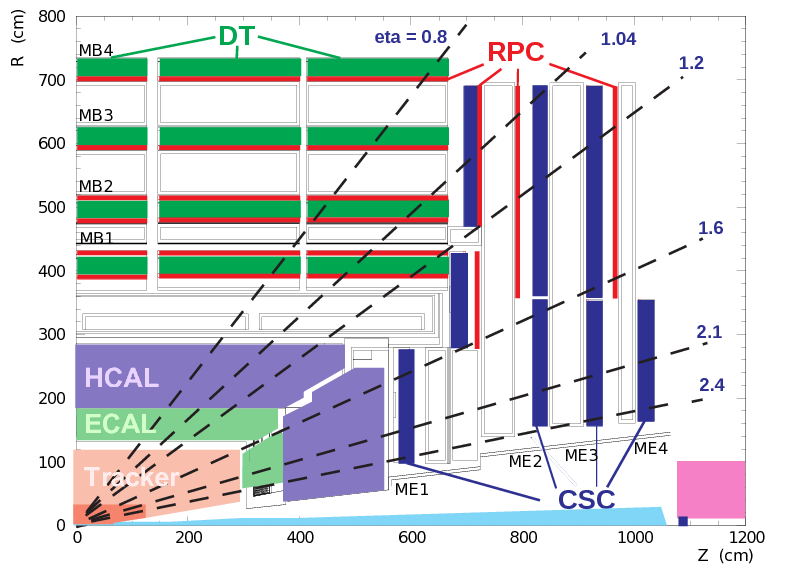
\includegraphics[width = 0.95 \textwidth]{Chapters/Chapter2_CERN/Figures/MuonSys-mod3.pdf}
 \caption{Cross section of one quarter of the CMS muon system.} \label{fig::MuonAndCMS}
\end{figure}

The central region of the muon system consists of four concentric layers which cover $\vert \eta \vert$ $<$ 1.2 and are equipped with drift tubes (DT) while the endcap part ($\vert \eta \vert$ $<$ 2.4) has four stations containing cathode strip chambers (CSC). The DTs are designed for the low rate which is expected in the barrel region and thus have a slower response time than the CSCs in the endcap. 
The spatial resolutions obtained for the two detector systems are similar, 80-120$\unit{\mu m}$ for the DTs and 40-150$\unit{\mu m}$ for the CSCs~\cite{MuonPerformance}.
%Even though the used technology is different for the barrel and endcap, similar resolutions should be obtained. As expected, the first data results provided a clear confirmation with a spatial resolution of  
For the pseudo-rapidity region $\vert \eta \vert$ $<$ 1.6 additional resistive plate chambers (RPC) are added in order to ensure a fast response with good time resolution. Since the RPCs were specifically designed for an accurate time measurement the spatial resolutions are of less importance, which is indeed reflected by the obtained spatial resolution of 0.8-1.2$\cm$. % for this type of gaseous detectors.

\subsection{Online event filtering} \label{subsec::L1HLT}
The Large Hadron Collider is designed to provide about 40 million bunch crossings per second during which multiple simultaneous proton-proton collisions can occur. Storing such a large amount of data is not feasible, hence the event rate should be drastically reduced by filtering out the seemingly interesting interactions. 
%Such a selection process is possible since the produced proton-proton collisions are actually dominated by a large bunch of low-energetic QCD events (\textit{Definitely true?}).
\\
This event filtering process is performed by a dedicated multi-layered trigger system responsible for reducing the bunch crossing rate of about 40$\unit{MHz}$ to roughly 100$\unit{kHz}$ during the first step and reduce the event rate further to the maximal rate of 400$\unit{Hz}$ that can be stored with the second step. The two layers of the CMS trigger system are complementary since the first trigger (Level-1 or L1) is designed to execute fast decisions while the second one (High-Level trigger or HLT) is capable of performing complex calculations in case of interesting events.
\\
The L1 trigger is mounted partially on the detector itself and has only access to information from the calorimeter and muon subsystems. Since this trigger layer should decide within 3.2$\unit{\mu s}$ whether an event looks promising enough to be analysed further, the processing of each bunch crossing is pipelined to avoid any dead-time regions. The accepted events are studied in detail by the HLT, which has access to the complete read-out data and has less stringent time constraints. In contrast to the L1 trigger which merely functions as a keep/reject switch, the HLT also serves as a labelling system that tags the selected events with the specific trigger requirements that were satisfied. This information can then later be used during the offline selection to split the events into dedicated datasets.

Even though the online triggering systems provides a radical reduction rate, CMS still requires a dedicated offline computing system to store, transfer and manipulate the unprecedented amounts of recorded data. Since the CMS collaboration prefers the recorded data to remain accessible throughout the entire lifetime of the experiment, a complex distributed system of large scale with a layered structure is needed.
\\
This computing system is set up as a collaboration between LHC experiments, computing centres and middleware providers and is referred by as the WorldWide LHC Computing Grid (WLCG). The adopted hierarchical structure contains one single Tier-0 centre at CERN, a handful of Tier-1 centres at large national computing facilities and several Tier-2 centres at partner universities. Hence the majority of the resources are hosted outside the CERN area. 
\\
The Tier-0 is mainly devoted to recording the detector information from the experimental site (RAW) and reconstruct the first datasets (RECO). It is the only one of the computing centres which is not accessible for analysis use. The following layer of Tier-1's provides storage of a second complete copy of the RAW data and allows more complex reconstruction algorithms for RECO samples. Finally the Tier-2 centres are designed to be used for final-stage analysis and for specialised activities which can be performed offline.

\subsection{CMS performance during Run-I data-taking} \label{subsec::CMSPerf}

The number of proton-proton interactions delivered by the LHC can differ from the number of interactions actually recorded by the experiments. 
Such a data loss can for example be caused by a technical malfunction in one of the detector's subsystems or by an unregulated overload of the trigger rate. However the overall performance of the CMS detector during the Run-I data-taking period, ranging from 2010 to 2012, was really good and any significant data-losses were avoided. 
The CMS detector reached an efficiency of 92.24$\%$, 90.98$\%$ and 93.52$\%$ for 2010, 2011 and 2012, respectively. 
For the 2012 run at $\sqrt{s}$ = 8$\TeV$ the comparison between the integrated luminosity delivered by the LHC and recorded by the CMS experiment can be found in Figure~\ref{fig::LumiEff}. This analysis will be performed using a total of $19.6 \fbI$ of integrated luminosity recorded by the CMS experiment.

\begin{figure}[h!t]
 \centering
 %\includegraphics[width = 0.325 \textwidth]{Chapters/Chapter2_CERN/Figures/int_lumi_per_day_cumulative_pp_2010.pdf}
 %\includegraphics[width = 0.325 \textwidth]{Chapters/Chapter2_CERN/Figures/int_lumi_per_day_cumulative_pp_2011.pdf}
 \includegraphics[width = 0.7 \textwidth]{Chapters/Chapter2_CERN/Figures/int_lumi_per_day_cumulative_pp_2012.pdf}
 \caption{Integrated luminosity delivered by the LHC and recorded by the CMS experiment during the 2012 data-taking at $\sqrt{s}$ = 8$\TeV$.} \label{fig::LumiEff}
\end{figure}

Afterwards the recorded data is validated by the offline Data Quality Monitoring (DQM) to ensure that it is suited for physics analysis. This largely automated tool determines whether all subdetectors were working properly during data-taking and monitors the reconstruction of the various physics objects.

